\newpage
%\appendix
\addtocontents{toc}{\protect\setcounter{tocdepth}{1}}
    \renewcommand\thefigure{\thesection.\arabic{figure}} %Number figure B1, B2, etc.
    \renewcommand{\thetable}{C.\arabic{table}} %Number tables B1, B2, etc.
    \setcounter{figure}{0} %Start numbering from 1   
    \setcounter{table}{0}


\section{Test of Methodology for Different Topic}\label{appsec_feminism}

To test our methodology for corpus construction, we select a different topic and a new period of time. We select the topic feminism and the period of time between March 9\textsuperscript{th} and 11\textsuperscript{th}, 2022 (we selected a short period of time to have quick results). After, we also tested the scripts to update the data considering the period from March 11\textsuperscript{th} to 13\textsuperscript{th}, 2022. So our final data set have the tweets that talk about feminism between March 9\textsuperscript{th} to 13\textsuperscript{th}, 2022. Here we present the final characteristics of this corpus and the same plots that we used to describe the immigration corpus. 

\begin{table}[H]
            %\footnotesize
            \centering
            
            \subfile{tabs/corpus_characteristics_feminism.tex}
            
            \caption{Corpus Characteristics, Feminism Corpus and Labeled Subsample}
            
            \floatfoot{\it 
            Notes: Unique words and hashtags can have duplicates across the subcategories ''left-leaning'', ''right-leaning'' or ''unlabeled''.
            \\ 
            Data Source: Retrieved from Twitter API, spanning the time frame Mar 9\textsuperscript{th}, 2022 -- Mar 13\textsuperscript{th}, 2022. Corpus includes tweets by Twitter users in Chile or Chilean nationals that mainly pertain to feminism.}
            \label{tab_corpora_characs_feminism}
        \end{table}
        
        \begin{figure}[H]
             \centering
             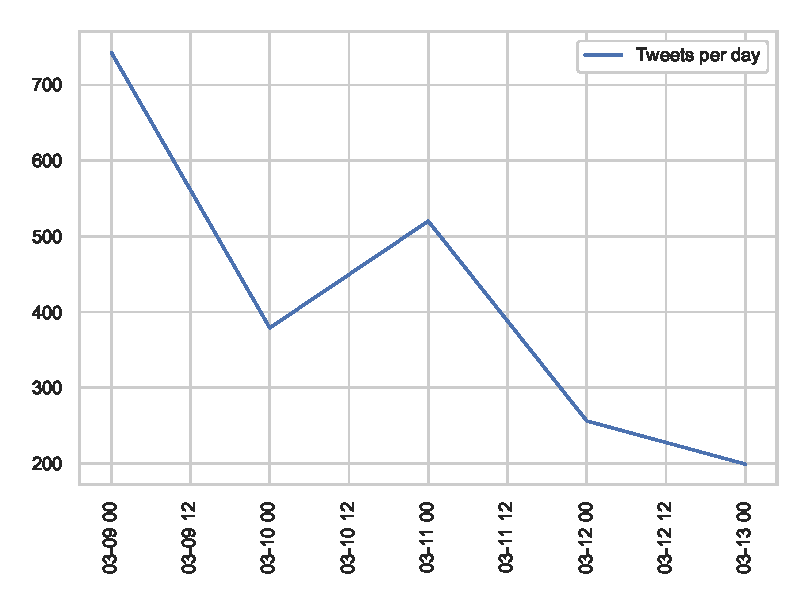
\includegraphics[width=.9\linewidth]{figs/Tweets_per_day_feminism.eps}
             \caption{Tweets per Day, Feminism Corpus}
             \label{total_tweets_per_day_feminism}
             \floatfoot{\it 
                    %Notes:  \\ 
                    Data Source: Retrieved from Twitter API, spanning the time frame Mar 9\textsuperscript{th}, 2022 -- Mar 13\textsuperscript{th}, 2022. Corpus includes tweets by Twitter users in Chile or Chilean nationals that mainly pertain to feminism.}
        \end{figure}
        
        
        \begin{figure}[H]
             \centering
             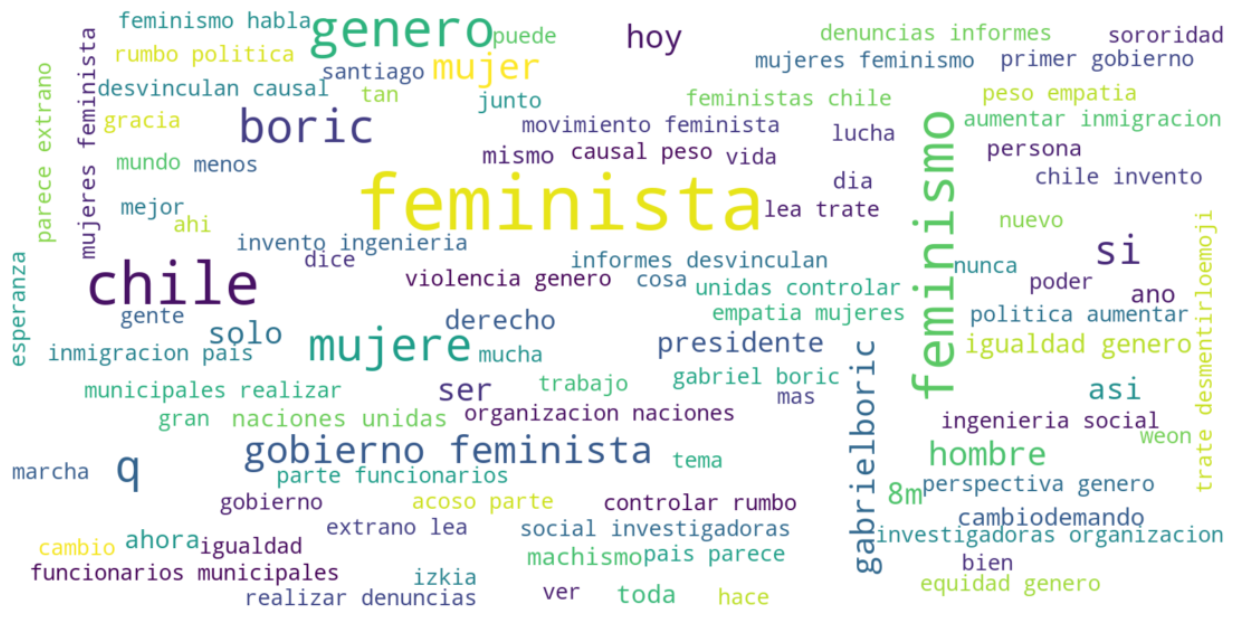
\includegraphics[width=.9\linewidth]{figs/wordcloud_feminism.png}
             \caption{Word Cloud of Tweets, Feminism Corpus}
             \label{feminism_Word_Cloud}
             \floatfoot{\it 
                    Notes:  Textual preprocessing steps include lowercase enforcement and converting Spanish special characters (e.g. á, ñ, etc.) into corresponding non-accentuated ones.
                    \\ 
                    Data Source: Retrieved from Twitter API, spanning the time frame Mar 9\textsuperscript{th}, 2022 -- Mar 13\textsuperscript{th}, 2022. Corpus includes tweets by Twitter users in Chile or Chilean nationals that mainly pertain to feminism.}
        \end{figure}
        
        \begin{figure}[H]
             \centering
             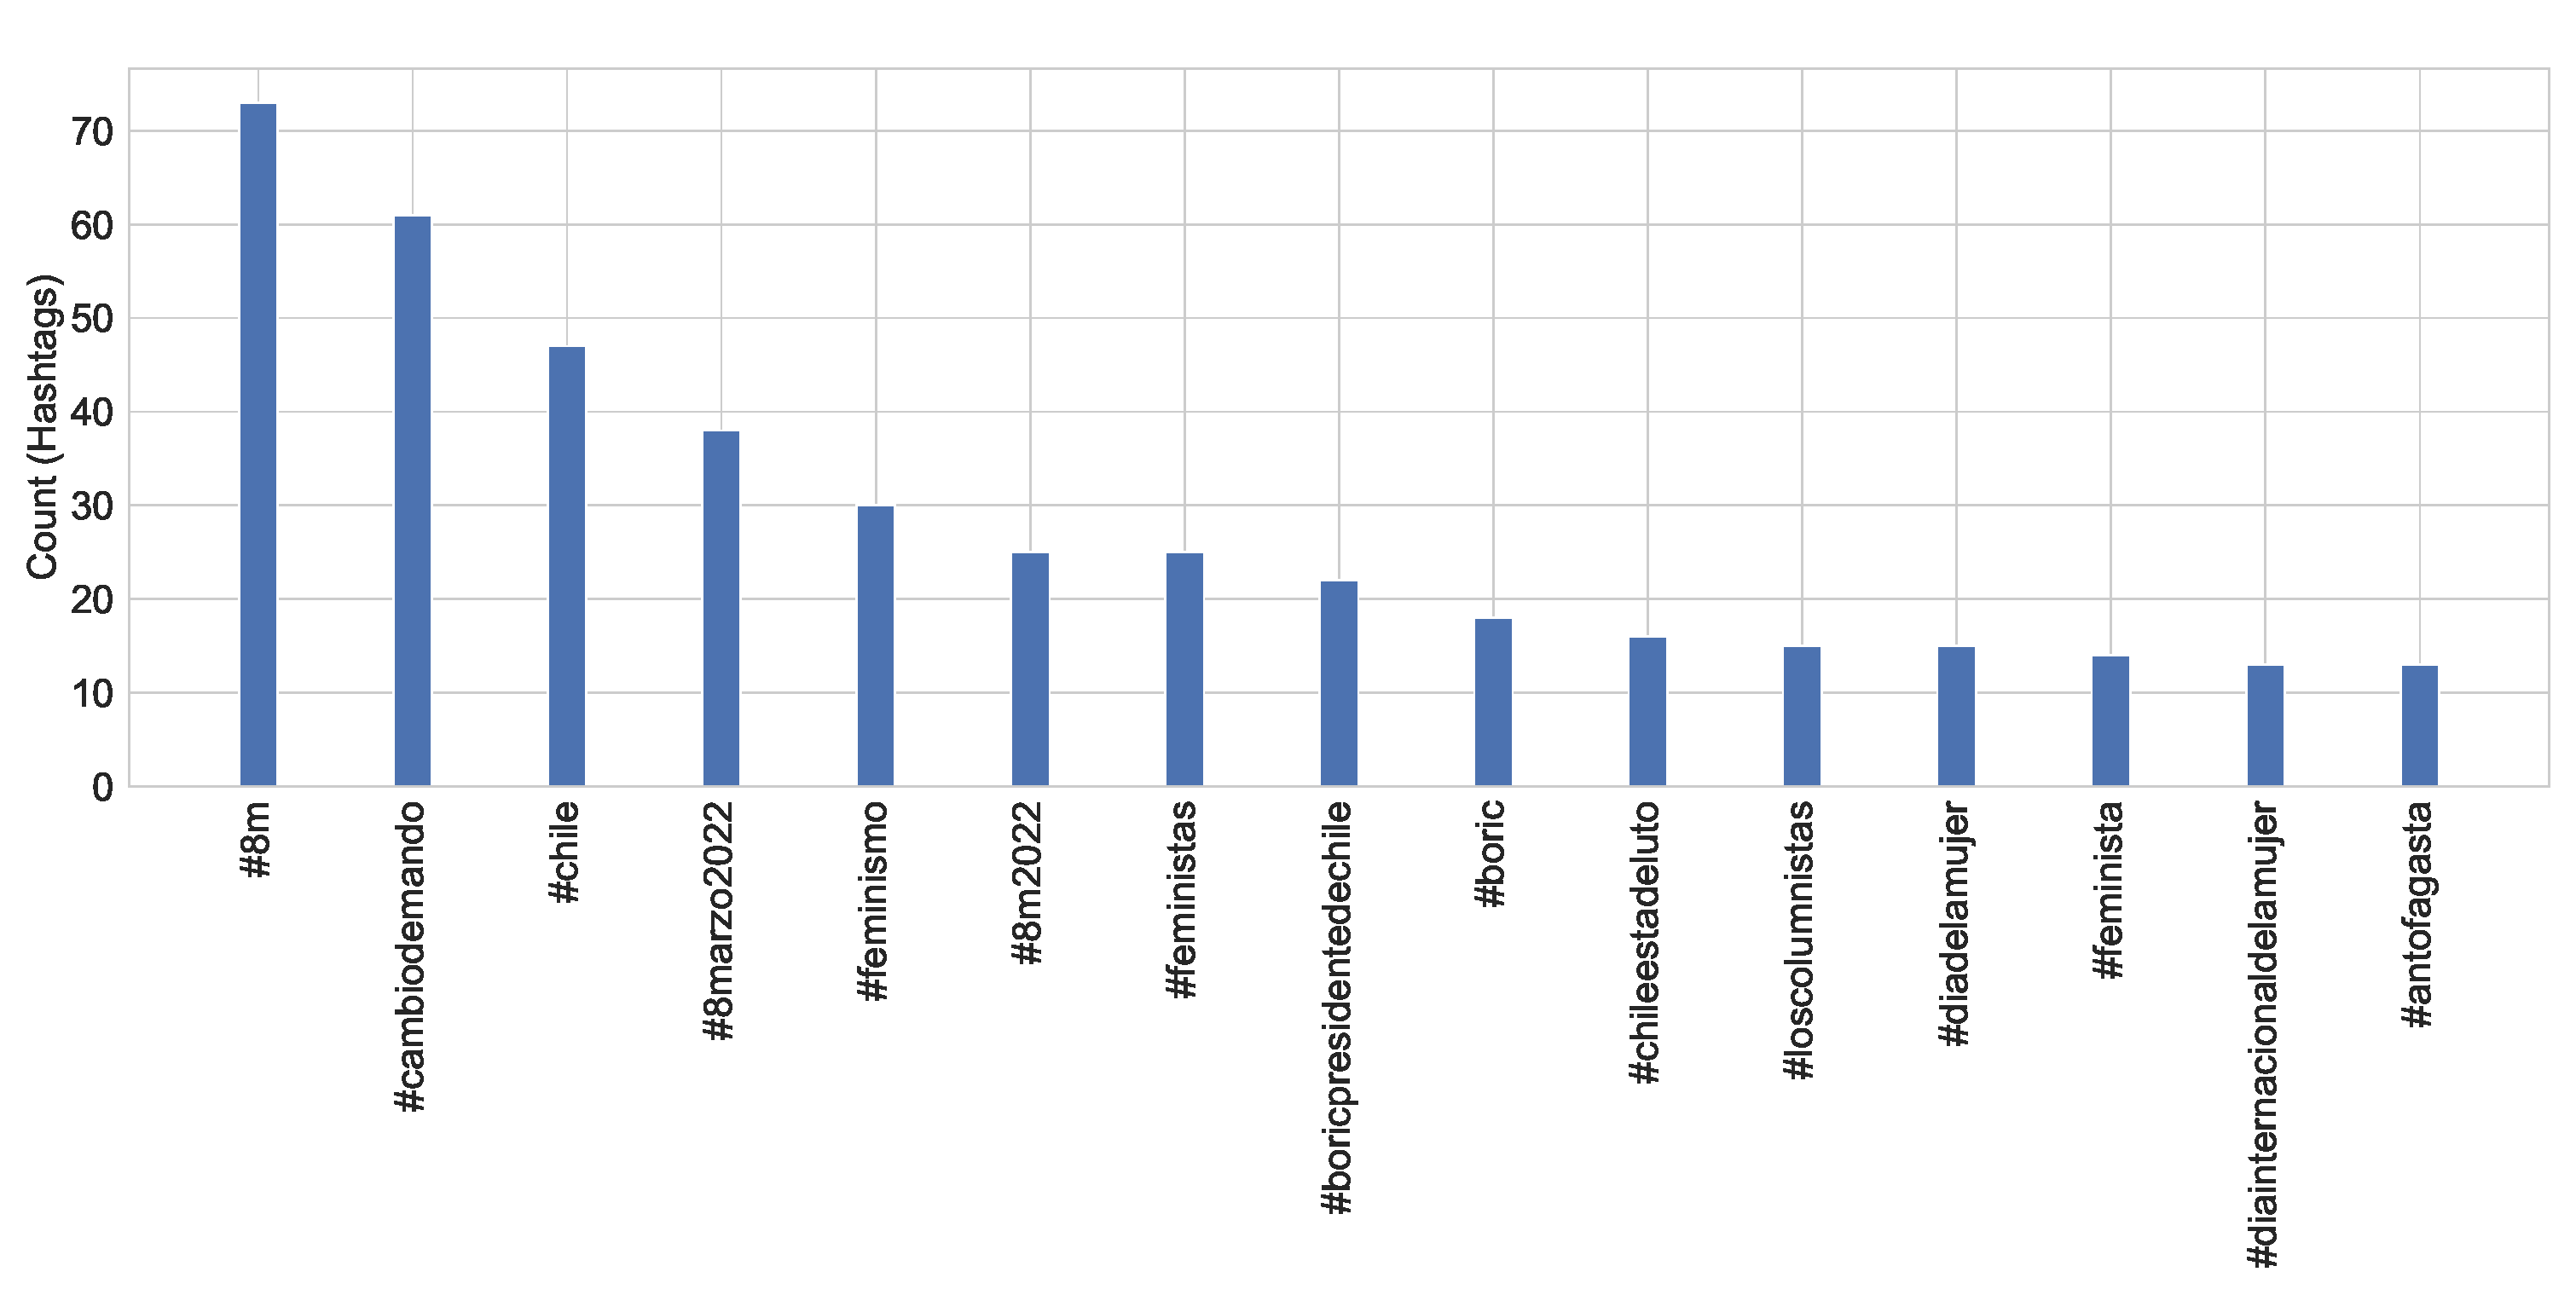
\includegraphics[width=.9\linewidth]{figs/Common_Hashtags_Feminism.eps}
             \caption{Top Hashtags, Feminism Corpus}
             \label{feminism_hashtags}
             \floatfoot{\it 
                    Notes:  Textual preprocessing steps include lowercase enforcement and converting Spanish special characters (e.g. á, ñ, etc.) into corresponding non-accentuated ones.
                    \\ 
                    Data Source: Retrieved from Twitter API, spanning the time frame Mar 9\textsuperscript{th}, 2022 -- Mar 13\textsuperscript{th}, 2022. Corpus includes tweets by Twitter users in Chile or Chilean nationals that mainly pertain to feminism.}
        \end{figure}
        
        \begin{figure}[H]
             \centering
             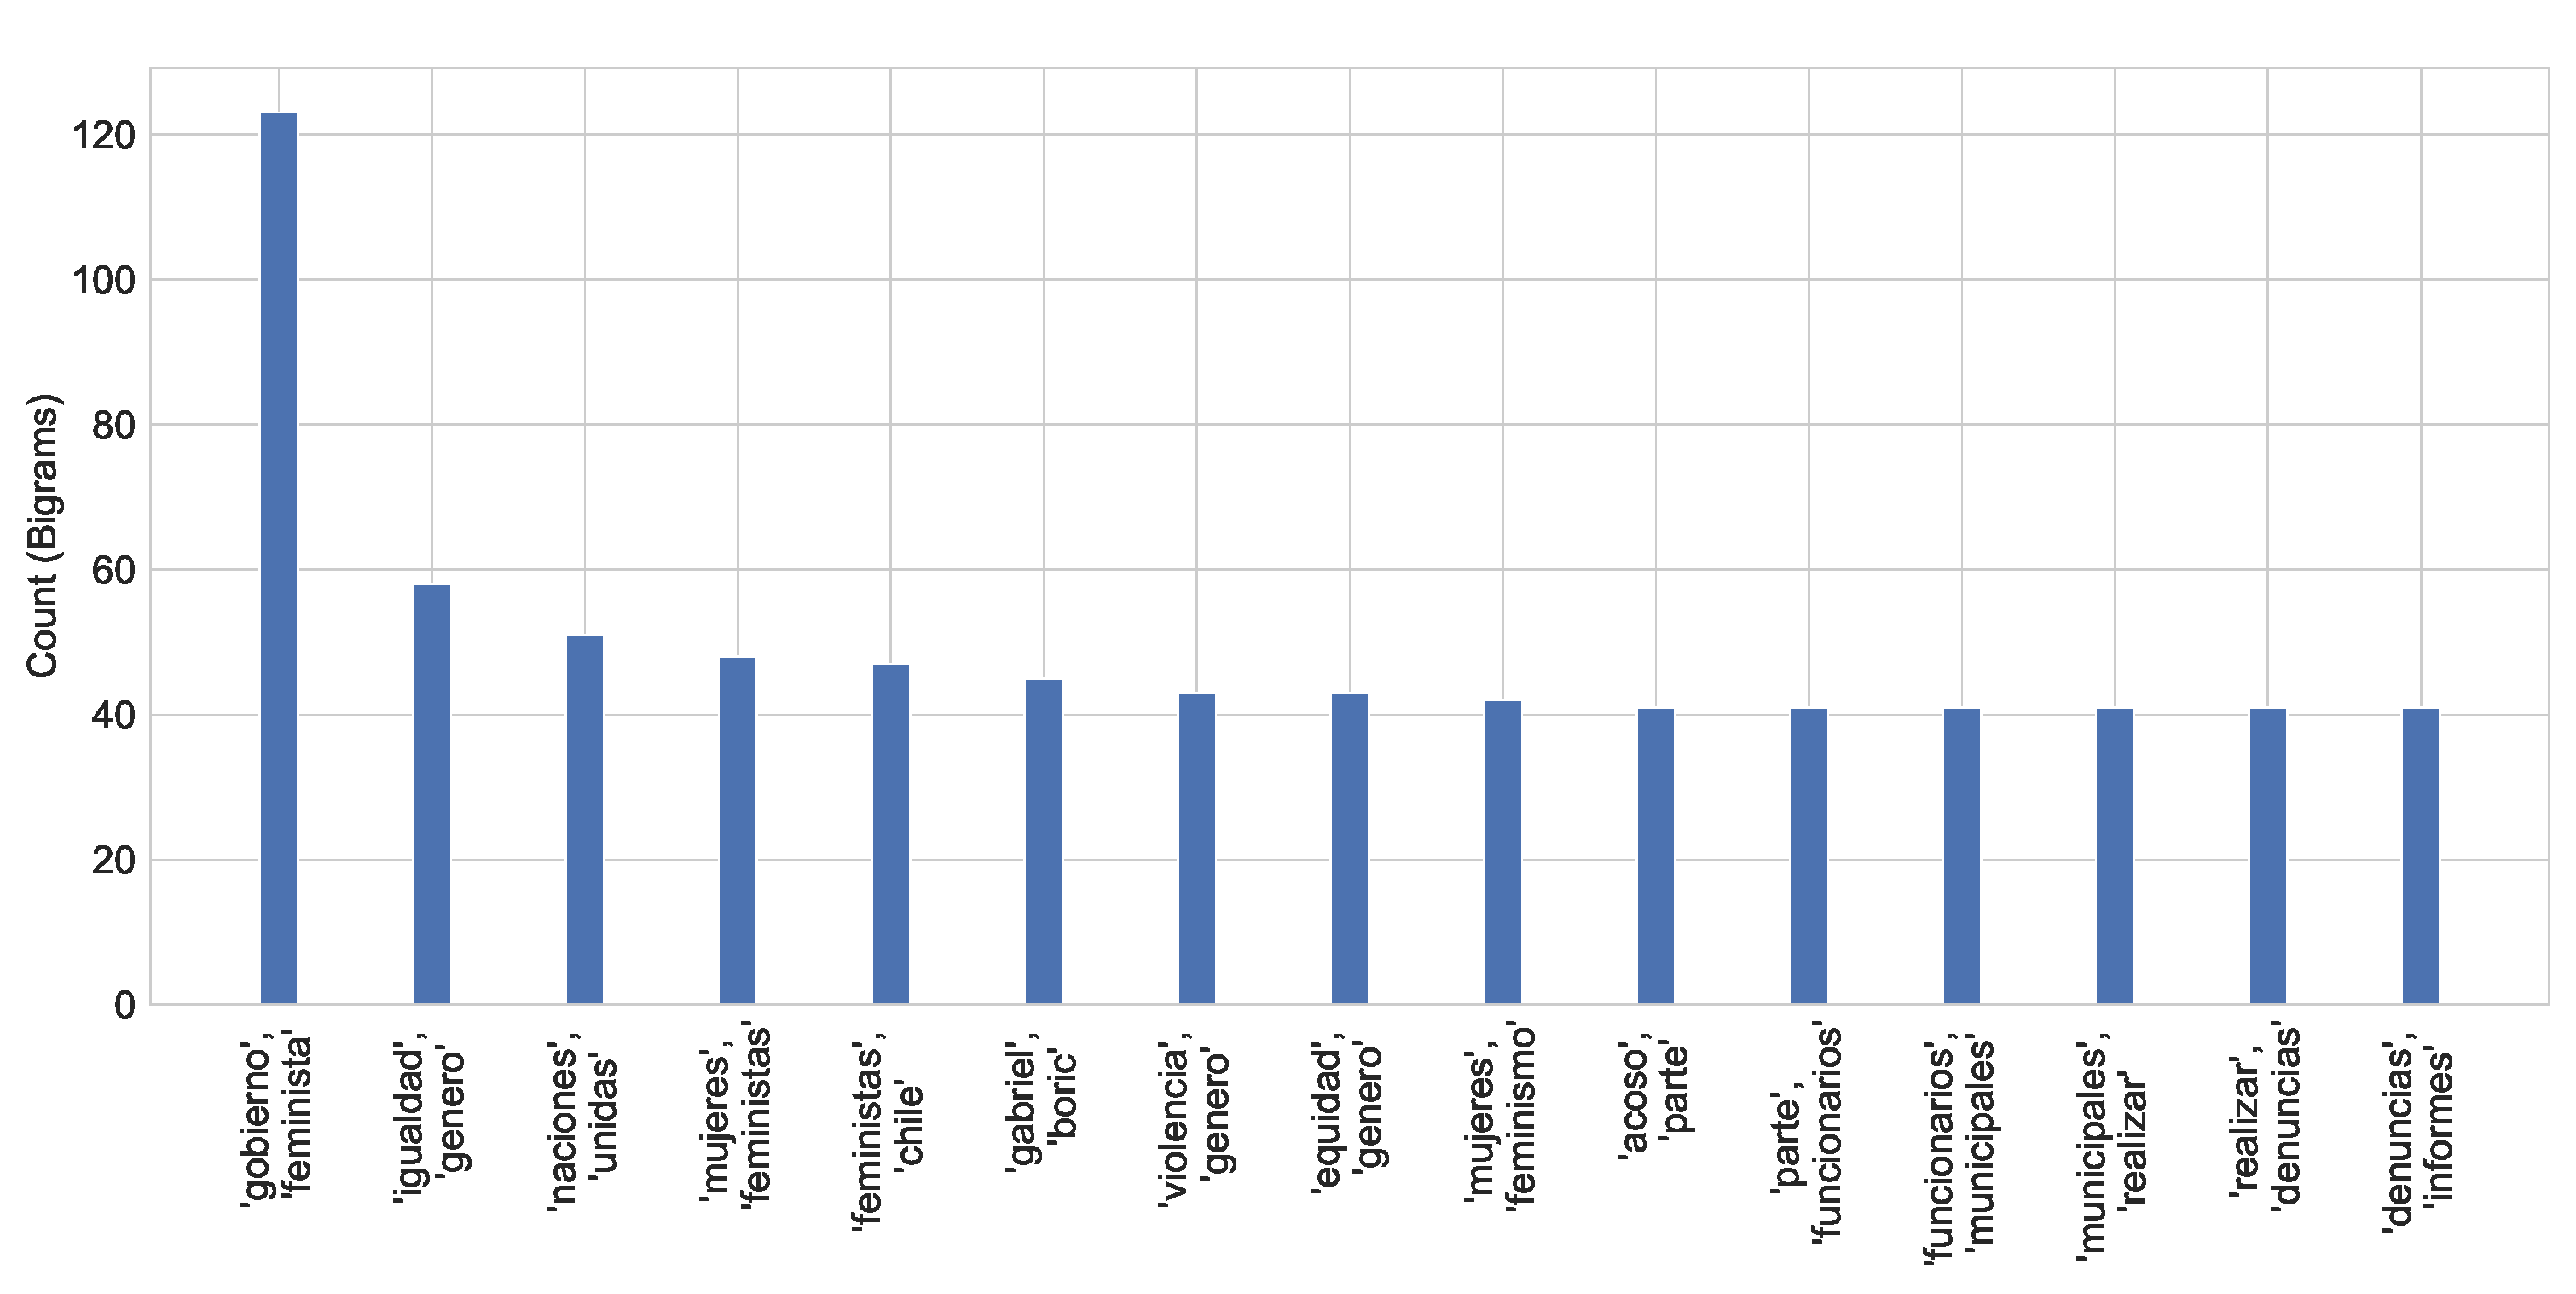
\includegraphics[width=.9\linewidth]{figs/Common_Bigrams_Feminism.eps}
             \caption{Top Bigrams, Feminism Corpus}
             \label{feminism_bigrams}
             \floatfoot{\it 
                    Notes:  Textual preprocessing steps include lowercase enforcement and converting Spanish special characters (e.g. á, ñ, etc.) into corresponding non-accentuated ones.
                    \\ 
                    Data Source: Retrieved from Twitter API, spanning the time frame Mar 9\textsuperscript{th}, 2022 -- Mar 13\textsuperscript{th}, 2022. Corpus includes tweets by Twitter users in Chile or Chilean nationals that mainly pertain to feminism.}
        \end{figure}

 